\subsection*{Molecule-level matching across generators}

\begin{figure}[p]
\centering
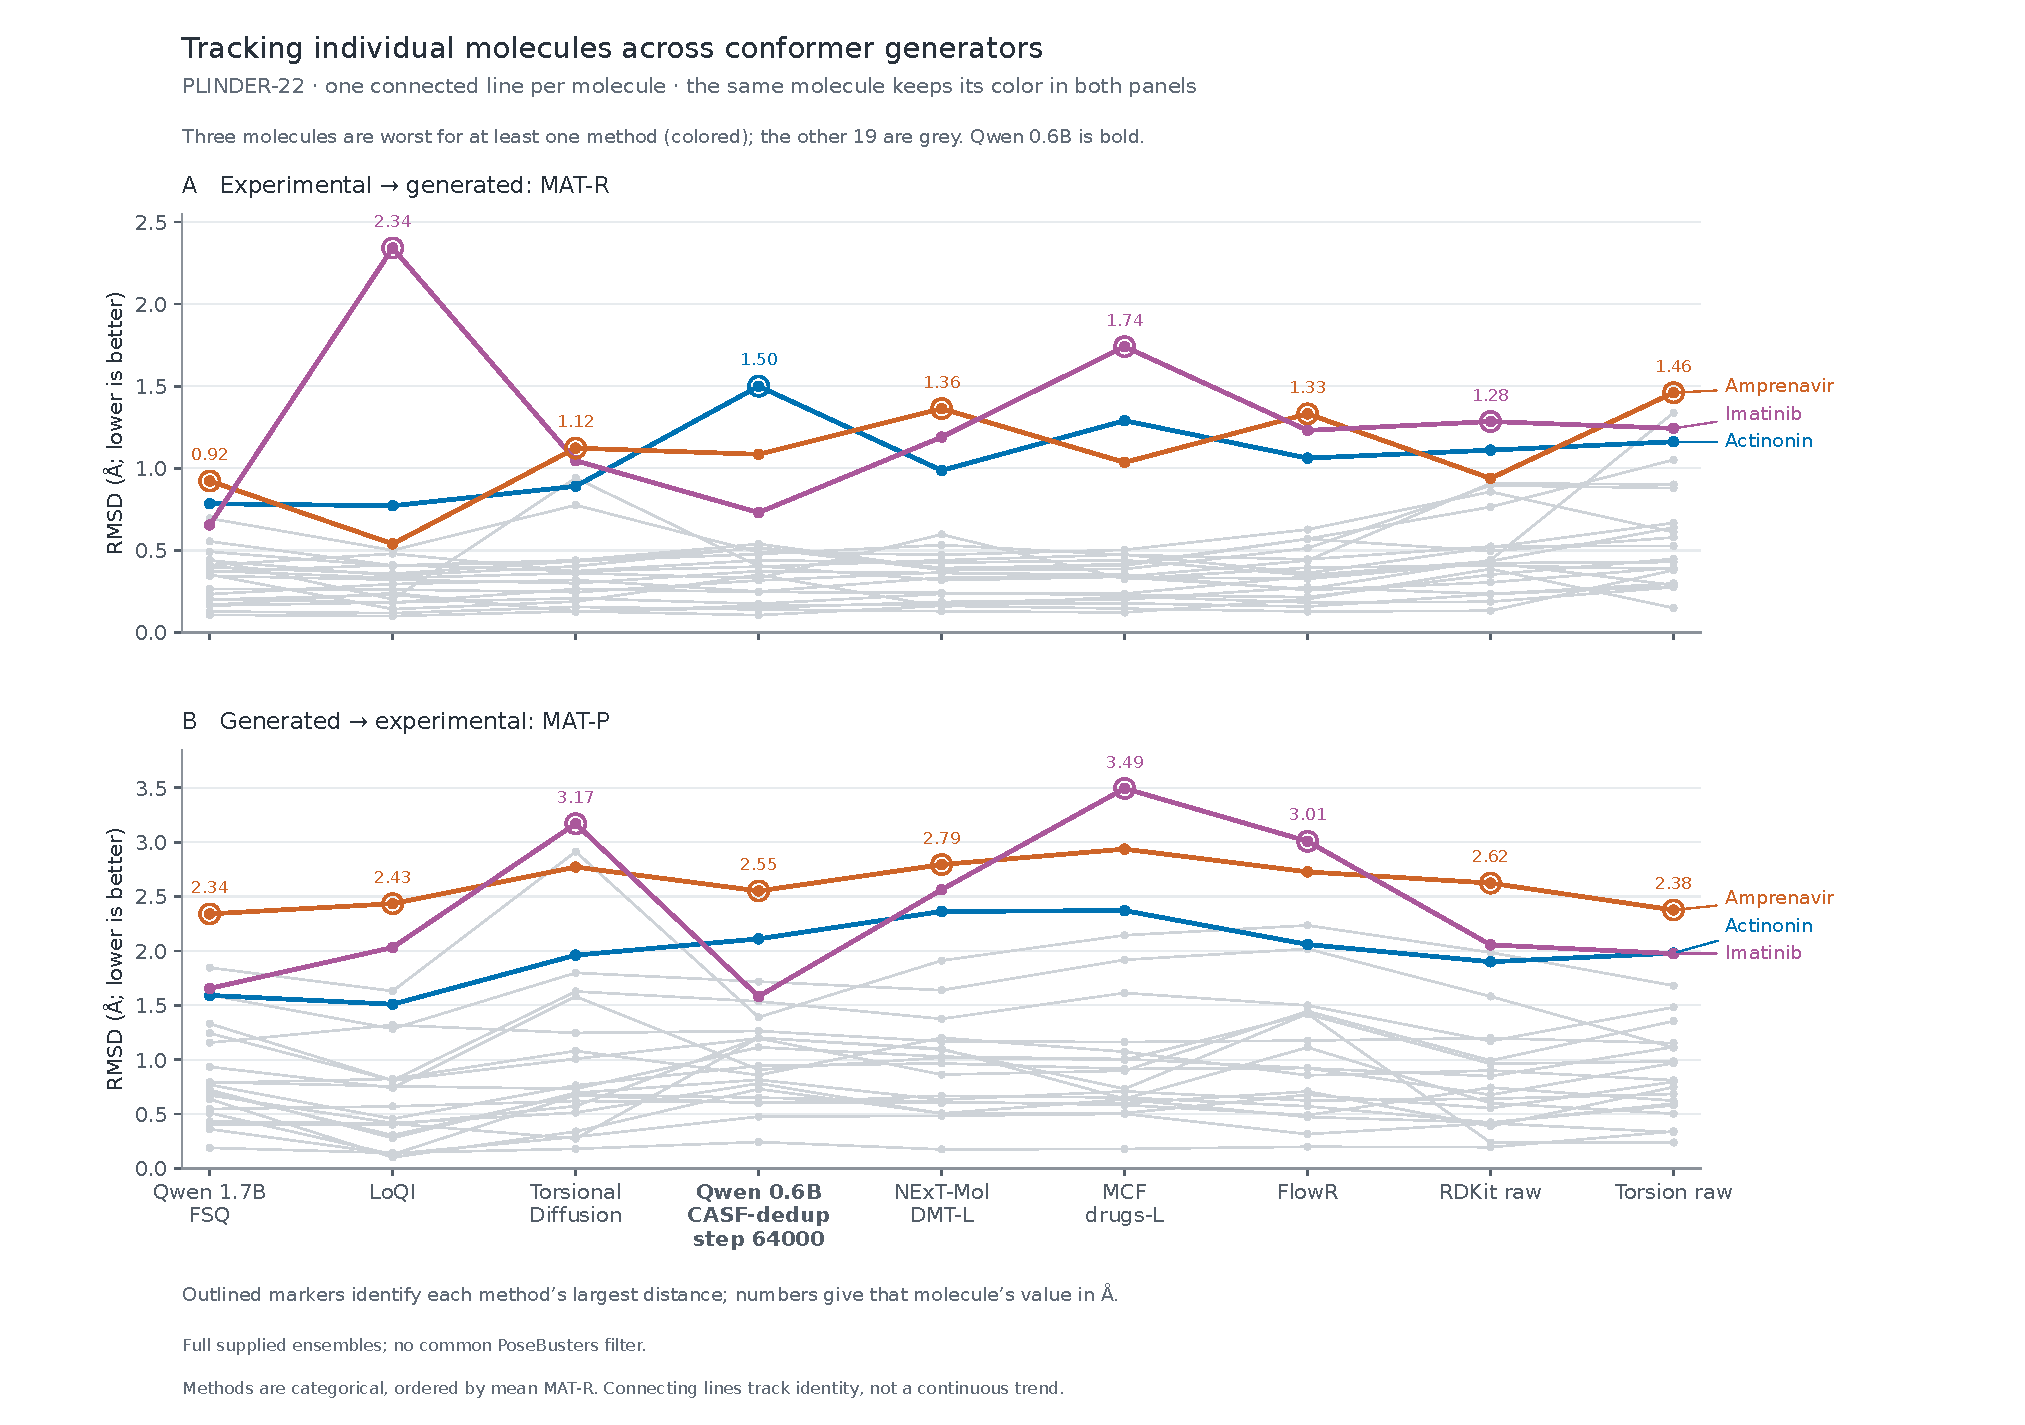
\includegraphics[width=\linewidth,height=0.74\textheight,keepaspectratio]{figures/figure-plinder-molecule-tracking.pdf}
\caption{Molecule-level matching distances on PLINDER-22. Each line follows one molecule across methods: (A) MAT-R and (B) MAT-P; lower is better. Colored lines identify the two molecules with the largest distance for at least one displayed method in either panel; grey lines show the other 20. Outlined markers identify each method's largest value. Methods are ordered by mean MAT-R. The comparison includes Qwen 1.7B FSQ, the five external learned generators, and the two raw classical baselines.}
\label{fig:plinder-molecule-tracking}
\end{figure}
